
% The \phantomsection command is needed to create a link to a place in the document that is not a
% figure, equation, table, section, subsection, chapter, etc.
% https://tex.stackexchange.com/questions/44088/when-do-i-need-to-invoke-phantomsection
\phantomsection

% Multiple-language document - babel - selectlanguage vs begin/end{otherlanguage}
% https://tex.stackexchange.com/questions/36526/multiple-language-document-babel-selectlanguage-vs-begin-endotherlanguage
\begin{otherlanguage*}{english}

% The \phantomsection command is needed to create a link to a place in the document that is not a
% figure, equation, table, section, subsection, chapter, etc.
% https://tex.stackexchange.com/questions/44088/when-do-i-need-to-invoke-phantomsection
\phantomsection

% Multiple-language document - babel - selectlanguage vs begin/end{otherlanguage}
% https://tex.stackexchange.com/questions/36526/multiple-language-document-babel-selectlanguage-vs-begin-endotherlanguage
\begin{otherlanguage*}{brazil}

\chapter{\lang{Experimental Analysis}{Análise Experimental}} \label{cap:analise:experimental}

Este capítulo apresenta a análise experimental sobre o Serviço criado. Para que seja possível
validar o Serviço uma aplicação de testes foi criada em Go, que é um acrescentador de valores
em memória, sempre que uma requisição chega a ele, este incrementa um no seu valor em memória.
Esta é uma aplicação \textit{Stateful} e, portanto, é passível de ser utilizada no nosso Serviço.
Este capítulo pretende responder a algumas perguntas a partir da análise dos experimentos:

\begin{itemize}
	\item Existe impacto ao se utilizar o Interceptador para interceptar requisições a
	aplicação alvo? Este impacto deve ser considerado ao se utilizar o Serviço nas
	aplicações.
	\item Qual o impacto de tempo para a aplicação ser restaurada quando analizado com
	o tempo do Kubernetes realizar a restauração de uma falha em um contêiner? Qual o
	impacto da adição da recuperação com técnicas de \textit{Event Sourcing}?
	\item Qual o impacto geral na vazão e latência da aplicação quando ela está sendo
	interceptada pelo Interceptador? Qual a vazão e latência da aplicação quando ela
	está sendo executada \textit{standalone}? Há um impacto pela adição do Interceptador?
	\item Qual a vazão e latência durante a recuperação da aplicação pelas técnicas de
	\textit{Event Sourcing}?
\end{itemize}

Para responder estas perguntas fizemos primeiro uma instrumentação no Serviço para que
pudessemos coletar pontos importante para análise, como, por exemplo, momentos em que a
aplicação alterou o estado do Interceptador, momento da introdução da falha do Interceptador,
momento da detecção pelo Administrador de Estado e tempo até a aplicação retornar ao estado
de Pronto. Análise de teste de carga para determinar a vazão e latência das requisições com
diferentes cargas no sistema. A partir disto pretendemos responder as perguntas para esta
análise. Também pontuasse que como a aplicação executa em um nó, as latências de rede não
impactam tanto nos dados obtidos.

Para realizar o teste de carga, utilizamos a aplicação bombardier \cite{bombardier}, ela
permite realizar um número arbitrário de requisições concorrentes, definindo a quantidade
de requisições e o tamanho da concorrência, isto nos permite testar a aplicação sobre uma
carga mais real. Para coleta de outras métricas utilizamos horário de início e fim de cada
uma das modificações, como o Serviço e a aplicação executam na mesma máquina o horário é
igual para todos e não é necessário sincronização de relógios entre máquinas.

\section{Análise aplicação standalone}

Na aplicação \textit{standalone}, isto é, sem interferência do nosso Serviço, executando
puramente no Kubernetes sem nosso Operador, temos o gráfico de vazão, N clientes realizando
requisições paralelamente durante 10 segundos, por latência, em millisegundos da Figura
\ref{fig:analysis-standalone}. Verificamos que a partir de mil e quinhentos clientes nossa
aplicação atinge seu limite, a partir do qual, qualquer acréscimo de requisições 
simultâneas, degrada a performance de latência e a qualidade de seriviço. O gráfico aponta
o p95 da latência das aplicações. Esta análise nos permite dar uma perspectiva sobre o
quão bom nosso Serviço pode ser, este é o melhor caso da aplicação, ou seja, não há nenhum
interferência de serviços externos, exceto o Kubernetes. Os pontos em destaque no gráfico
da Figura \ref{fig:analysis-standalone} são nossos pontos de controle para os testes.

\begin{figure}[h]
\centering
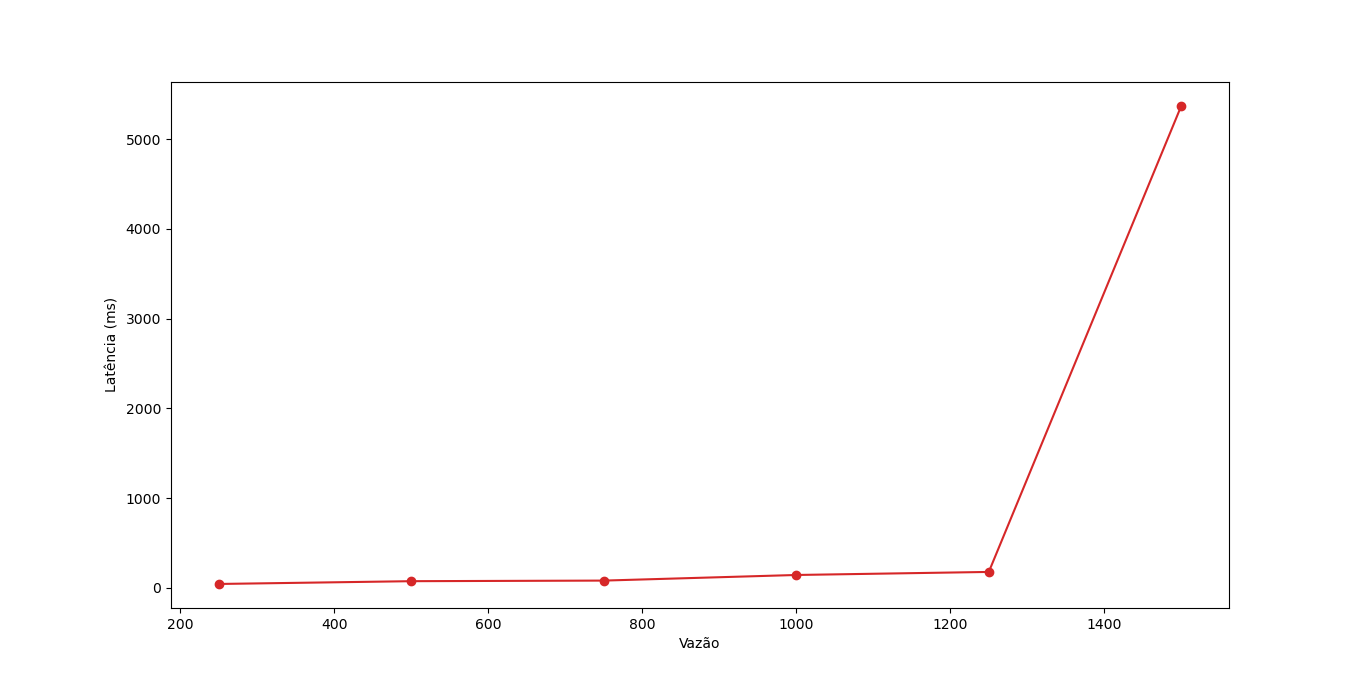
\includegraphics[scale=0.46]{images/standalone_graph.png}
\caption{Gráfico de vazão X latência da aplicação alvo executando de forma \textit{standalone}.}
\label{fig:analysis-standalone}
\end{figure}

\section{Análise do Interceptador na aplicação}

A partir do momento que integramos a aplicação alvo no nosso Operador esperamos ter um
acréscimo do tempo de latência da aplicação e também um limite menor a partir do momento
em que a aplicação atinge o pico de vazão. Realizando os mesmos testes com pontos de controle
a cada duzento e cinquenta clientes com requisições simultâneas temos o gráfico da Figura
\ref{fig:analysis-interceptor}, verificamos que a aplicação perde performance, no ponto de
controle de quinhentos clientes já atingimos o mesmo pico da aplicação \textit{standalone}
mostrado na \ref{fig:analysis-standalone}.

\begin{figure}[h]
\centering
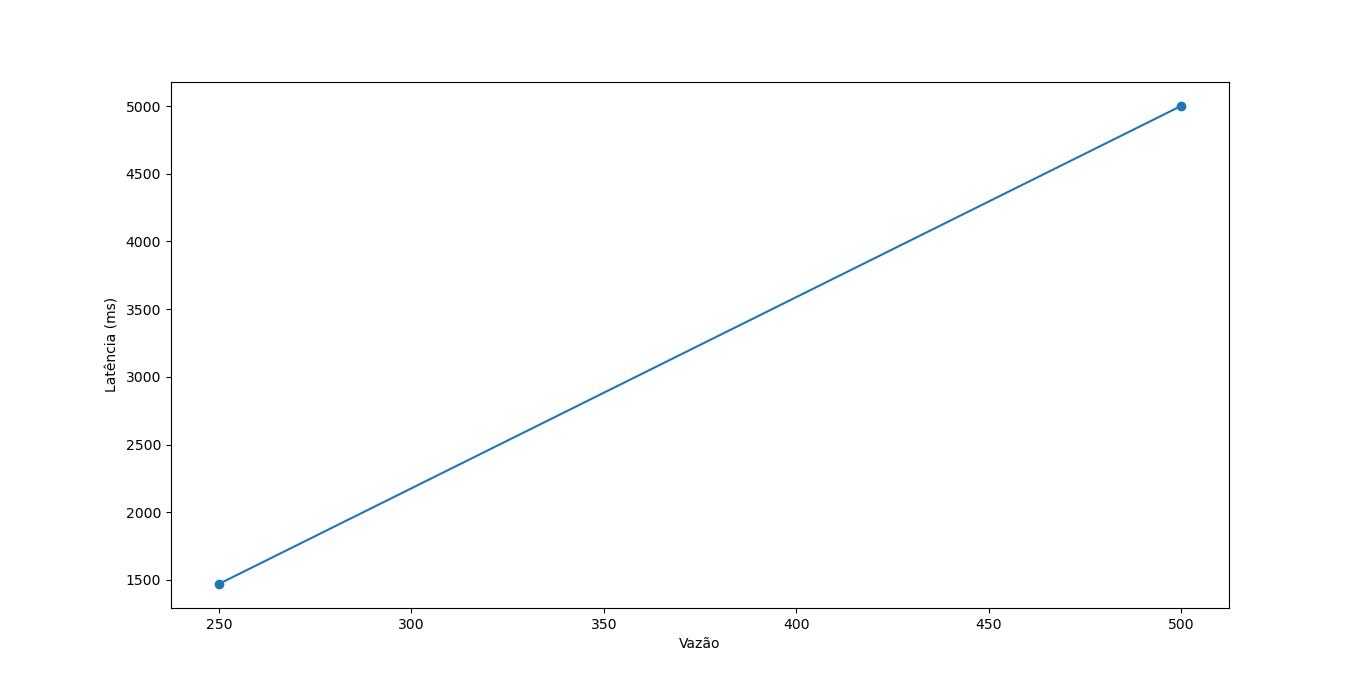
\includegraphics[scale=0.46]{images/interceptor_graph.png}
\caption{Gráfico de vazão X latência da aplicação alvo com o Interceptador.}
\label{fig:analysis-interceptor}
\end{figure}

No gráfico da Figura \ref{fig:analysis-interceptor-standalone} temos a sobreposições 
dos gráficos de latência da aplicação alvo sem o Operador e com o Operador. O gráfico
deixa mais claro a perda de performance, já que logo no primeiro ponto de control de
duzentos e cinquenta clientes temos uma latência de 44.42ms para a aplicação
\textit{standalone} e de 1470ms para a aplicação com o Operador. A diferença dos valores
se deve a todas as operações que realizamos no Interceptador, como adição ao banco de
dados da requisição interceptada e encaminhamento da requisição para a aplicação alvo.
A perda já é evitada por ambos os contêineres estarem executando no mesmo Pod e reduzindo
as camadas necessárias para transferência dos dados via TCP.

\begin{figure}[h]
\centering
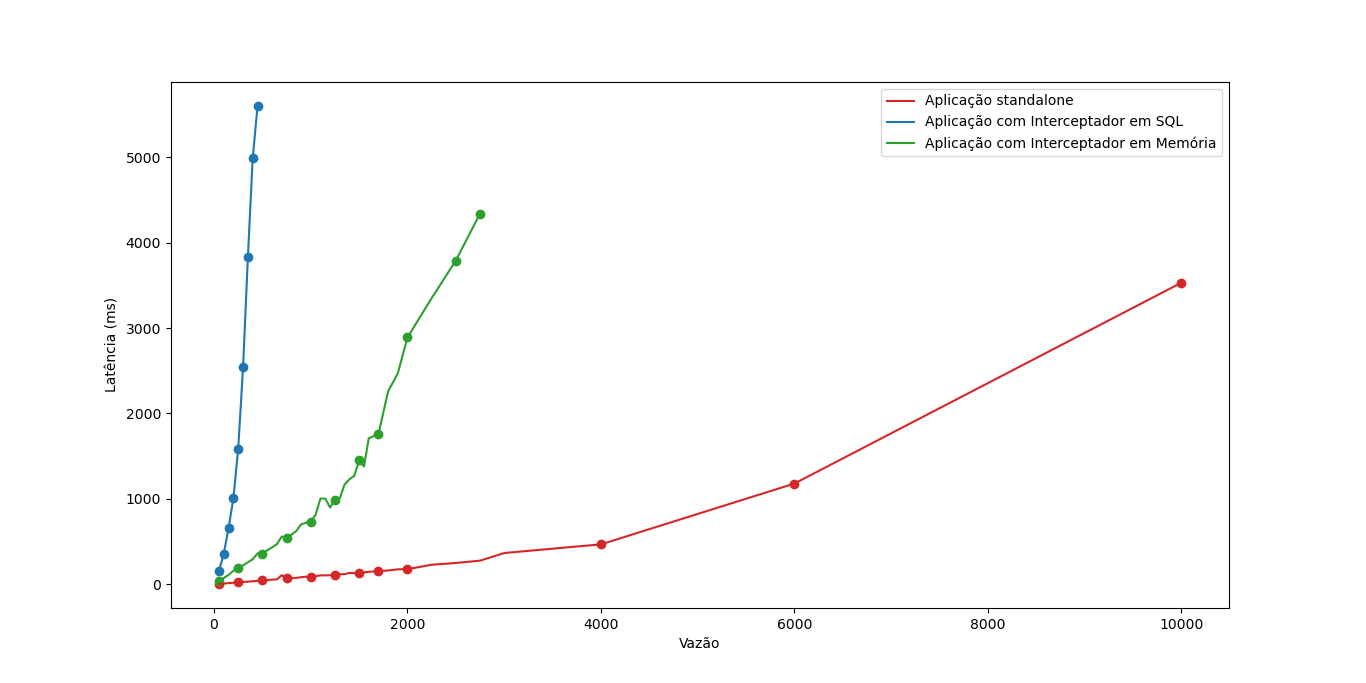
\includegraphics[scale=0.46]{images/vazaoxlatencia.png}
\caption{Gráfico de sobreposição de vazão X latência da aplicação alvo de forma \textit{standalone} e da aplicação alvo com o Interceptador.}
\label{fig:analysis-interceptor-standalone}
\end{figure}

Poderíamos melhorar a performance do Interceptador com banco de dados mais personalizado para
nossa aplicação com adição de índices ou utilização de cache. Entretanto, estes fatores não
foram cobridos no nosso trabalho.

\section{Análise do período de Checkpoint do Interceptador}

Nesta Seção, pretendemos discutir e analisar qual o tempo gasto pelo \textit{Checkpoint} do
Interceptador na implementação com CRIU. Na implementação com técnicas de
\textit{Event Sourcing} não temos uma alteração, por exemplo, da latência das requisições ao
se fazer um \textit{Checkpoint}, pois este ocorre passivamente. Já na implementação com CRIU
a aplicação deve ser pausada por um momento para salvamento do seu estado e isto gera uma
piora na qualidade de serviço para o usuário de maneira momentânea. Para simular este estado,
iniciamos realizando um teste de carga na aplicação para criar um estado, a partir daí, iniciamos
ao mesmo tempo um \textit{Checkpoint} a partir do Interceptador e um outro teste de carga, que deve
durar mais tempo que o \textit{Checkpoint}.

Coletamos dados para a latência das requisições que atingem o Interceptador em um período de
tempo que inclui antes de uma falha na aplicação alvo, durante a recuperação da aplicação
alvo e posteriormente da recuperação no mesmo teste. Estes testes nos proveram uma latência
média de 7.3s para as requisições do período de tempo, onde já existiam mil requisições
acumuladas para que ocorresse a reprojeção durante a recuperação e os tínhamos cem clientes
realizando mil requisições simultâneas para a aplicação durante o período de tempo.

Novamente, tivemos uma piora de latência do serviço, isto se deve principalmente pelo fator
da nossa aplicação ter que realizar todas as requisições já feitas para a aplicação atingir
o estado antes da falha na recuperação. Na proposta de \cite{muller2022architecture} a
arquitetura realiza a poda das requisições, onde, menos requisições teriam que ser refeitas
a partir de uma falha para a recuperação através da criação de imagens de \textit{Checkpoint}
utilizando o CRIU.

\section{Análise da recuperação com técnicas de Event Sourcing}

Nesta Seção queremos investigar o impacto das técnicas de \textit{Event Sourcing} na
recuperação do estado de uma aplicação que falhou. Para isso, primeiro utilizamos nosso teste
de carga para levar a aplicação até um estado, com mil requisições(caso A), dez mil
requisições(caso B) e vinte mil requisições(caso C), com mais requisições acumuladas o serviço
degrada a ponto de não possibilitar testes com as configurações de \textit{cluster} que utilizamos.
Depois repetimos o mesmo teste com cada uma delas, ao alcançar o estado a aplicação terá uma falha
ocasionada pela interrupção da execução do container pela ferramenta crictl. Após a falha,
a recuperação deve ocorrer, neste momento, passamos a realizar um teste de carga igual para
todos os casos, cem requisições serão feitas de maneira concorrente entre dez clientes.

\begin{table}[htb]
\caption[Latência durante recuperação de requisições acumuladas.]{Latência durante recuperação de requisições acumuladas.}
\label{tab:event-sourcing-latency}
\centering
\begin{tabular}{|c|c|}
\hline
\textbf{\begin{tabular}[c]{@{}c@{}}Ńúmero de requisições\\ acumuladas\end{tabular}} & \textbf{Latência} \\ \hline
1000(A)                                                                            & 74.69ms             \\ \hline
10000(B)                                                                            & 122.76ms            \\ \hline
20000(C)                                                                               & 10010ms             \\ \hline
\end{tabular}
\end{table}

Os resultados do teste estão na Tabela \ref{tab:event-sourcing-latency}. Verificamos, que,
temos uma degradação relevante entre dez mil requisições acumuladas e vinte mil requisições
acumuladas, indo de 122.76ms de latência para 10010ms de latência para as requisições.
Novamente, quanto mais requisições acumuladas o Interceptador possui, mais demorada se torna
uma recuperação ao realizar todas as requisições novamente para a aplicação alvo. Esta análise
mostra uma premissa que já tínhamos, de que existe um limite para utilização das técnicas
de \textit{Event Sourcing} sobre o \textit{Checkpoint/Restore}, já que, conforme mais tempo
a aplicação vive, mais se torna necessário utilizar outras técnicas para ser possível reduzir
a replicação das requisições na recuperação, em \cite{muller2022architecture} a diminuição da
pilha foi feita através da implementação da recuperação com CRIU.

Agora, pretendemos também investigar o tempo que levamos entre a detecção, a recuperação e
atingir o estado de pronto em cada caso, como em \cite{vayghan2021kubernetes}, adicionamos
métricas ao controlador de Pods, para definir a detecção, e no nosso script identificamos o
início da falha, a recuperação é definida nos momentos em que se altera o estado do Interceptador
e o estado de Pronto também é instrumentado pelo controlador de Pods. Na Tabela
\ref{tab:latency-restoring} temos os valores para o início da recuperação após uma falha e o tempo
até a aplicação estar disponível novamente após a recuperação. No caso C temos um tempo muito
superior aos casos A e B, isto se deve por vários fatores, desde a configuração do nosso
\textit{cluster} que não permite escalabilidade e também da necessidade de se obter todas as
requisições de um banco de dados para replicação das requisições. A Tabela \ref{tab:latency-restoring}
demonstra que a implementação com técnicas de \textit{Event Sourcing} degrada conforme temos mais
requisições acumuladas no Interceptador para realizar a recuperação.

\begin{table}[htb]
\caption[Tempos de identificação de recuperação e de recuperação final de um contêiner alvo.]{Tempos de identificação de recuperação e de recuperação final de um contêiner alvo.}
\label{tab:latency-restoring}
\centering
\begin{tabular}{|c|c|c|}
\hline
\textbf{\begin{tabular}[c]{@{}c@{}}Ńúmero de requisições\\ acumuladas\end{tabular}} & \textbf{\begin{tabular}[c]{@{}c@{}}Tempo de Identificação \\ (microssegundos) \end{tabular}} &
\textbf{\begin{tabular}[c]{@{}c@{}}Tempo de Recuperação \\ (microssegundos) \end{tabular}} \\ \hline
1000(A) &  991011 & 990702 \\ \hline
10000(B) & 998153 & 975395     \\ \hline
20000(C) & 1013021 & 85667000000 \\ \hline
\end{tabular}
\end{table}

\end{otherlanguage*}
